\newpage
\textbf{Ejemplo 8}\\
Supongamos que un inversionista desea adquirir la aceptación bancaria del ejemplo anterior, la cual figura con una tasa de registro del 30\% periódico 40 días vencido y con precio de registro $P_r =  97,65 COP$ pero él también sabe que para adquirirla deberá pagar una comisión a un corredor de bolsa lo cual hará variar el precio que él debe pagar y también la rentabilidad que él pueda obtener. Supongamos que la comisión que cobra un corredor por la compra es del 0,475\% periodo 40 días periodo vencido ¿Cuál es el precio del inversionista Pc =  ? COP , que incluye la comisión del comisionista vendedor, el precio de registro y la comisión de bolsa del comprador. El punto de referencia es el precio de registro $P_r$ ¿Cuál es la rentabilidad del inversionista $i_c =? \%?$ periódica 40 días vencido, o $j=? \hspace{0.5mm} nadv$
%\newpage %USAR SOLO SI EL SOLUCIÓN QUEDA SOLO Y ES NECESARIO BAJARLO A LA SIGUIENTE PAGINA

\textbf{Solución.}
%La tabla ira centrada
\begin{center}
 \renewcommand{\arraystretch}{1.5}% Margenes de las celdas
 %Creación de la cuadricula de 3 columnas
 \begin{longtable}[H]{|p{0.5\linewidth}|p{0.5\linewidth}|}
  %Creamos una linea horizontal
  \hline
  %Definimos el color de la primera fila
  \rowcolor[HTML]{FFB183}
  %%%%% INICIO ASIGNACIÓN FECHA FOCAL %%%%%%%
  %%%%%%%%%% INICIO TITULO
  %Lo que se hace aquí es mezclar las 3 columnas en una sola
  \multicolumn{2}{|c|}{\cellcolor[HTML]{FFB183}\textbf{1. Asignación período focal}}                  \\ \hline
  %%%%%%%%%% FIN TITULO
  %%%%% INICIO DECLARACIÓN DE VARIABLES %%%%%%%
  \multicolumn{2}{|c|}{$pf = 40 \textit{ pdv}$}                                                     \\ \hline
  %%%%%%%%%% INICIO TITULO
  %Lo que se hace aquí es mezclar las 3 columnas en una sola
  \multicolumn{2}{|c|}{\cellcolor[HTML]{FFB183}\textbf{2. Declaración de variables}}                \\ \hline
  %%%%%%%%%% FIN TITULO
  %%%%%%%%%% INICIO DE MATEMÁTICAS
  %Cada & hace referencia al paso de la siguiente columna
  $i_c = 30\% -0,475\% = 29,525\% \hspace{1mm} p40dv$ & $P_R=?$                                     \\
  $P_c =  ? COP$                                         &                                             \\
  $n= \frac{40}{365} \hspace{1mm} p(40das) $          &                                             \\ \hline
  %%%%%%%%%% FIN DE MATEMÁTICAS
  %%%%% FIN DECLARACIÓN DE VARIABLES

  \rowcolor[HTML]{FFB183}
  \multicolumn{2}{|c|}{\cellcolor[HTML]{FFB183}\textbf{3. Diagrama de flujo de caja}}               \\ \hline
  \multicolumn{2}{|c|}{ 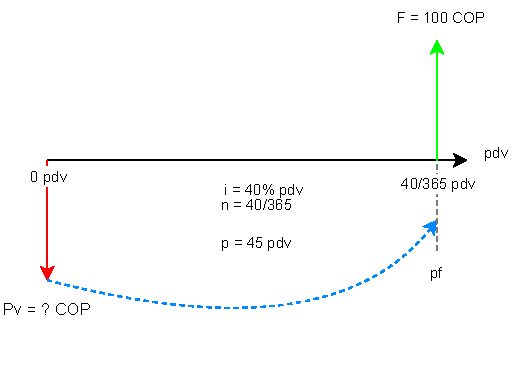
\includegraphics[trim=-78 0 -78 0]{3_Capitulo/img/ejemplos/8/capitulo3ejercicio8.pdf} }  \\ \hline
  %%%%% INICIO FLUJO DE CAJA
  \rowcolor[HTML]{FFB183}
  \multicolumn{2}{|c|}{\cellcolor[HTML]{FFB183}\textbf{4. DECLARACIÓN de formulas}}                 \\ \hline
  %Mezclamos 3 columnas y pondremos el dibujo
  %%%%%%%%%%%%% INSERCIÓN DE LA IMAGEN
  %Deberán descargar las imágenes respectivas del drive y pegarlas en la carpeta
  %n_capitulo/img/ejemplos/1/capitulo1ejemplo1.pdf  (el /1/ es el numero del ejemplo)
  \multicolumn{2}{|c|}{ $P = F(1 + i)^n $ Valor presente }                                          \\ \hline
  %%%%%%%%%%%%% FIN INSERCIÓN DE IMAGEN
  %%%%%FIN FLUJO DE CAJA


  %%%%%% INICIO DESARROLLO MATEMÁTICO
  \rowcolor[HTML]{FFB183}
  %%%%%%%%%%INICIO TITULO
  \multicolumn{2}{|c|}{\cellcolor[HTML]{FFB183}\textbf{5. Desarrollo matemático}}                   \\ \hline
  %%%%%%%%%% FIN TITULO
  %%%%%%%%%% INICIO MATEMÁTICAS
  \multicolumn{2}{|C{\linewidth}|}{
  $P_c =  100 COP(1 + 0,29525)\frac{40}{365} = 97,204 COP$ Ecuación de valor

  $P_R = 0,972047( 5{.}000{.}000 COP) =  4{.}860{.}245 COP$

  $P_c - P_R =  4{.}860{.}235 COP -  4{.}858{.}285 COP = 1{.}950 COP$
  }                                                                                                 \\ \hline

  %%%%%%%%%% FIN MATEMÁTICAS
  %%%%%% FIN DESARROLLO MATEMÁTICO
  %%%%%% INICIO RESPUESTA
  \rowcolor[HTML]{FFB183}
  %%%%%%%%%%INICIO TITULO
  \multicolumn{2}{|c|}{\cellcolor[HTML]{FFB183}\textbf{6. Respuesta}}                               \\ \hline
  %%%%%%%%%% FIN TITULO
  %%%%%%%%%% INICIO RESPUESTA MATEMÁTICA
  \multicolumn{2}{|C{\textwidth}|}{
  $P_R =  4{.}860{.}245 COP$
  }                                                                                                 \\ \hline


  %%%%%%%%%% FIN MATEMÁTICAS
  %%%%%% FIN RESPUESTA
 \end{longtable}
 %Se crean dos lineas en blanco para que no quede el siguiente texto tan pegado
 %\newline \newline %USARLO SI CREES QUE ES NECESARIO
\end{center}